\documentclass[submit,techrep,noauthor]{ipsj}

\usepackage[dvipdfmx]{graphicx}
\usepackage{latexsym}

\begin{document}

\title{DPDKのRun-to-Completionモデルを用いた\\L2分散計算環境の提案}

\affiliate{NITech}{名古屋工業大学大学院\\Nagoya Institute of Technology}
\author{山本 竜也}{Yamamoto Tatsuya}{NITech}
\author{川島 龍太}{Kawashima Ryota}{NITech}
\author{松尾 啓志}{Matsuo Hiroshi}{NITech}

\begin{abstract}
  分散計算環境で実行される処理の中には,与えられたデータを繰り返し用いながら,小さいデータを計算機間でやりとりする処理がある.例えば,単回帰分析やロジスティック回帰などの機械学習である.これらの処理において,TCP/IPによる制御は相対的に大きなオーバーヘッドとなる.また,カーネルによるパケットI/O処理はDPDKのパケットI/O処理に比べて低速である.本研究では,DPDKのRun-to-Completionモデルを用いたL2分散計算環境を提案する.計算機間の通信にDPDKによるL2通信を用いることによって,TCP/IPによる通信のオーバーヘッドを低減するとともに,カーネルによるパケットI/O処理に比べて高速なパケットI/O処理を用いることができる.また,Run-to-Completionモデルを採用することによって,Pipelineモデルを用いる場合に比べてCPUリソースやL1キャッシュを有効活用できる.送られてきた32個の値を加算し送り返すプログラムを用いた事前実験2では,提案手法を用いた場合の処理性能はTCP/IPによる通信を用いた場合に比べて,内部ループ回数が1回の場合は30倍,10回の場合は4倍,100回の場合は0.4倍高いことを確認した.また,単回帰分析を行うプログラムを用いた評価では,提案手法を用いた2台での分散処理の実行時間は,1台での集中学習の場合に比べて2倍,TCP/IPによる通信を用いた2台での分散処理の場合に比べて1.2倍高速であることを確認した.
\end{abstract}

\begin{jkeyword}
  分散計算環境,DPDK,Run-to-Completion,L2通信,L1キャッシュ
\end{jkeyword}


\maketitle

\section{はじめに}
\label{sec:Background}
分散計算環境で実行される処理の中には,与えられたデータを繰り返し用いながら,L2フレームより小さいデータを計算機間でやりとりする処理がある.例えば,単回帰分析やロジスティック回帰などの機械学習である.これらの処理において,TCP/IPによる制御はオーバーヘッドである.また,カーネルによるパケットI/O処理には,一定時間に受信するパケットの量が増えると,コンテキストスイッチが増加して,割り込み以外の処理が実行できなくなるといった問題があり,DPDKのパケットI/O処理に比べて低速である.

DPDKにはRun-to-CompletionモデルとPipelineモデルの2つのモデルがある.Run-to-Completionモデルは受信処理,パケット処理,送信処理を一つの論理コアで行い,Pipelineモデルは受信処理,パケット処理,送信処理をそれぞれ別の論理コアで行う.Pipelineモデルはそれぞれの処理が論理コアを専有するため,CPUリソースやL1キャッシュを有効活用できない.

そこで本研究では,DPDKのRun-to-Completionモデルを用いたL2分散計算環境を提案する.計算機間の通信にDPDKによるL2通信を用いることによって,TCP/IPによる通信のオーバーヘッドを低減するとともに,カーネルによるパケットI/O処理に比べて高速なパケットI/O処理を用いることができる.また,Run-to-Completionモデルを採用することによって,Pipelineモデルを用いる場合に比べてCPUリソースやL1キャッシュを有効活用できる.

なお,本研究が提案する分散計算環境には3つの前提を設ける.1つ目の前提はL2通信が可能であるローカルなクラスタ環境で動作することである.2つ目の前提は計算機間でやりとりされるデータのサイズはL2フレームより小さいことである.3つ目の前提は各計算機で実行される処理はイテレーションが多いもので,その実行に必要なデータは小規模であることである.これらの前提は特に機械学習では満たされることが多いと考える.

本稿の構成は以下のとおりである.第\ref{sec:Problem}章で分散計算環境の問題点を述べ,第\ref{sec:DPDK}章でDPDKについて説明する.第\ref{sec:Proposed}章で提案手法について述べ,第\ref{sec:PreExperimentOne}章,第\ref{sec:PreExperimentTwo}章,第\ref{sec:Evaluation}章で提案手法の事前実験と評価を行う.第\ref{sec:RelatedWorks}章で関連研究を述べ,第\ref{sec:Conclusion}章でまとめと今後の課題を述べる.

\section{分散計算環境の問題点}
\label{sec:Problem}
本章では,分散計算環境の問題点としてTCP/IPによる制御とカーネルによるパケットI/O処理について述べる.

\subsection{TCP/IPによる制御}
TCP/IPによる通信ではルーティング,誤り制御,順序制御といった制御が行われる.ルーティングとは端末の相互接続関係や各端末間の通信回線の混み具合の情報を取得し,送信元端末から宛先端末までのルートを決定する制御である.本研究が提案する分散計算環境はL2通信が可能であるローカルなクラスタ環境で動作するため,ルーティングは必ずしも必要ではない.誤り制御とはデータが伝送中に誤ったり失われたりしたとき,それを回復して受信側に正しいデータを送り届ける制御である.本研究が提案する分散計算環境の各計算機で実行される処理はイテレーションが多用され,多少のパケットロスであれば処理結果に影響を与えない,また明らかな異常値は処理時に排除することも可能であるため,誤り制御も必ずしも必要ではないと考える.順序制御とは受信データの重複をなくし,正しい順序に並び替える制御である.本研究が提案する分散計算環境の計算機間でやりとりされるデータのサイズはL2フレーム(ジャンボフレームを含む)より小さいため,順序制御も必ずしも必要ではない.

よって,TCP/IPによる制御は本研究が提案する分散計算環境においてはオーバーヘッドであるため,本研究はTCP/IPによる通信ではなくL2通信を用いることにした.

\subsection{カーネルによるパケットI/O処理}
Linux2.6以前のカーネルによるパケットI/O処理(図\ref{fig:KernelPacketIO})では,パケットを受信するたびにNIC(Network Interface Card)からのハードウェア割り込みが発生する.そのため,一定時間に受信するパケットの量が増えると,コンテキストスイッチが増加して,割り込み以外の処理時間が相対的に少なくなる.また,ユーザ空間からカーネル空間にはアクセスできないため,ユーザ空間のアプリケーションがパケットにアクセスするには,受信したパケットをカーネル空間からユーザ空間にコピーしなければならない.

パケット受信時のハードウェア割り込みを削減するために,Linux2.6以降のカーネルにはNAPI(New API)と呼ばれる仕組みが導入された.NAPIではパケット受信によるハードウェア割り込みが発生すると,NICからのハードウェア割り込みを一時的に無効化し,NICのデバイスドライバの挙動を割り込み駆動からポーリング駆動に切り替える.そして,処理すべきパケットがなくなるまでポーリング駆動で処理を行い,通常の割り込み駆動に戻る.

\begin{figure}[htb]
  \centering
  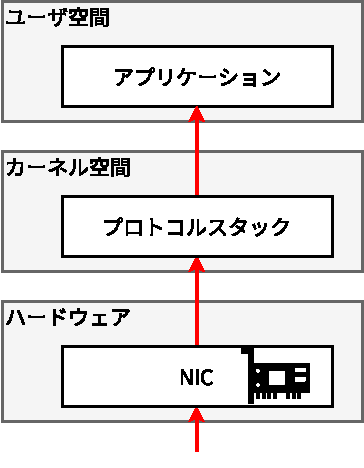
\includegraphics[width=0.5\columnwidth]{pictures/KernelPacketIO.pdf}
  \caption{カーネルによるパケットI/O処理}
  \label{fig:KernelPacketIO}
\end{figure}

\section{DPDK(Data Plane Development Kit)}
\label{sec:DPDK}
本章では,DPDKによるパケットI/Oとその実行モデルについて述べる.また,カーネルによるパケットI/OとDPDKによるパケットI/Oの比較やDPDKによるパケットI/Oの問題点についても述べる.

\subsection{DPDKによるパケットI/O}
DPDK \cite{DPDK} とは2010年にIntelによって作られたパケット処理を高速化するためのライブラリである.

DPDKは特定のCPUコアを占有することによって,NICを常時ポーリングで監視する.そのため,DPDKによるパケットI/O(図\ref{fig:DPDKPacketIO})では,一定時間に受信するパケットの量が増えると,コンテキストスイッチが増加して,割り込み以外の処理ができなくなってしまう問題は発生しない.

また,DPDKによるパケットI/Oでは,NICは受信したパケットをユーザ空間からアクセス可能な主記憶領域に書き込む.そのため,受信したパケットをカーネル空間からユーザ空間にコピーしなくても,ユーザ空間のアプリケーションがパケットにアクセスすることができる.

\begin{figure}[htb]
  \centering
  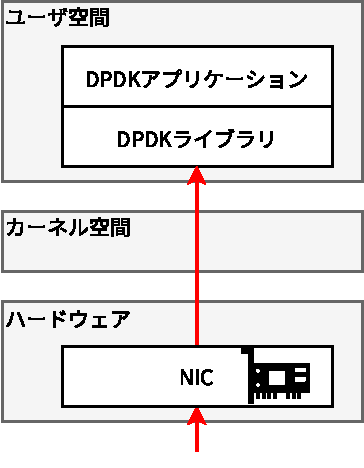
\includegraphics[width=0.5\columnwidth]{pictures/DPDKPacketIO.pdf}
  \caption{DPDKによるパケットI/O}
  \label{fig:DPDKPacketIO}
\end{figure}

\subsection{DPDKの実行モデル}
DPDKの実行モデルにはRun-to-CompletionモデルとPipelineモデルの二つがある.Run-to-Completionモデルは受信処理,パケット処理,送信処理を一つの論理コアで行うモデルである(図\ref{fig:RunToCompletion}).パケット処理が重たいと受信処理にCPUリソースが割当たらなくなり,パケットロスが生じてしまうため,パケット処理ではパケットヘッダの書き換えといった軽い処理が一般的には行われる.Pipelineモデルは受信処理,パケット処理,送信処理をそれぞれ別の論理コアで行うモデルである(図\ref{fig:Pipeline}).受信処理を行う論理コアとパケット処理を行う論理コアが別であるため,パケット処理が重たくてもパケットロスが生じることはない.しかし,CPUのL1キャッシュを有効活用できない.また,それぞれの処理が論理コアを占有するため,分散計算環境においてはコアの使用効率が悪い.

\begin{figure}[htb]
  \centering
  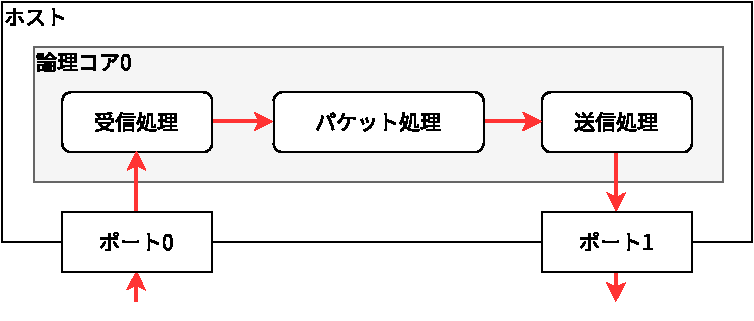
\includegraphics[width=\columnwidth]{pictures/RunToCompletion.pdf}
  \caption{Run-to-Completionモデル}
  \label{fig:RunToCompletion}
\end{figure}

\begin{figure}[htb]
  \centering
  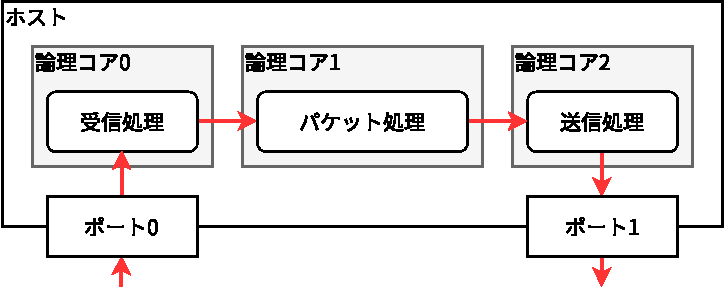
\includegraphics[width=\columnwidth]{pictures/Pipeline.pdf}
  \caption{Pipelineモデル}
  \label{fig:Pipeline}
\end{figure}

\subsection{パケットI/Oの比較}
文献 \cite{XDP} で調査された,カーネルによるパケットI/OとDPDKによるパケットI/Oの通信スループットを図\ref{fig:PacketIOComparison}に示す.このグラフの横軸は使用したCPUコアの数,縦軸は受信したパケットをすべてドロップしたときのスループットを表している.また,緑の折れ線はDPDKによるパケットI/O,ピンクの折れ線はカーネルによるパケットI/Oを表している.グラフより,DPDKのスループットはカーネルのスループットに比べて最大8倍程度高いことがわかる.

\begin{figure}[htb]
  \centering
  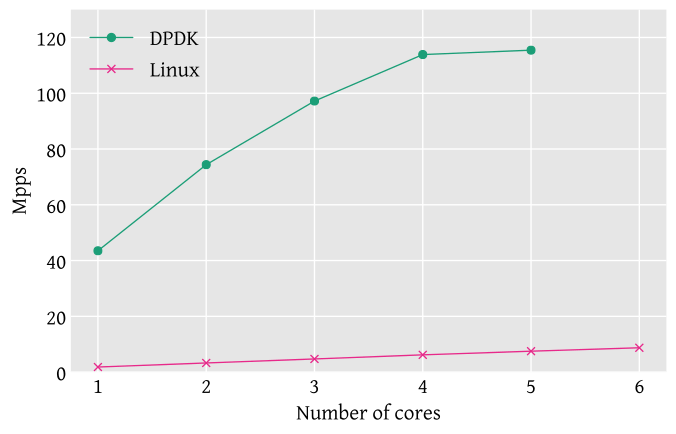
\includegraphics[width=\columnwidth]{pictures/PacketIOComparison.png}
  \caption{パケットI/Oの比較}
  \label{fig:PacketIOComparison}
\end{figure}

\subsection{DPDKによるパケットI/Oの問題}
DPDKは特定のCPUコアを専有することによって,NICを常時ポーリングで監視するため,通信スループットが低いときでもCPUリソースを無駄に使ってしまう.文献 \cite{XDP} で調査された,カーネルによるパケットI/OとDPDKによるパケットI/OのCPU使用率を図\ref{fig:DPDKProblem}に示す.このグラフの横軸は通信スループット,縦軸はCPU使用率を表している.また,緑の折れ線はDPDKによるパケットI/O,青の折れ線はカーネルによるパケットI/Oを表している.グラフから,カーネルによるパケットI/OのCPU使用率は通信スループットが高くなるにしたがって徐々に増えていくことがわかる.それに対して,DPDKによるパケットI/OのCPU使用率は通信スループットにかかわらず常に100\%であることがわかる.

\begin{figure}[htb]
  \centering
  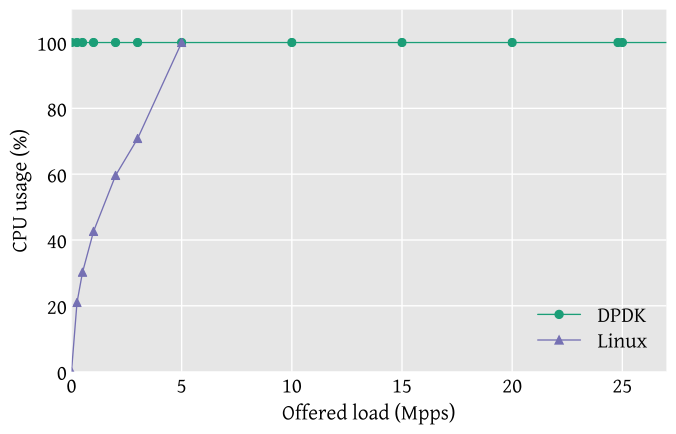
\includegraphics[width=\columnwidth]{pictures/DPDKProblem.png}
  \caption{DPDKによるパケットI/Oの問題}
  \label{fig:DPDKProblem}
\end{figure}

\section{提案手法}
\label{sec:Proposed}
本研究はDPDKのRun-to-Completionモデルを用いたL2分散計算環境を提案する.本章では,その概要としてDPDKによるL2通信を用いることとRun-to-Completionモデルを採用することについて述べる.

\subsection{DPDKによるL2通信の使用}
第\ref{sec:Problem}章で述べたとおり,TCP/IPによる通信ではルーティング,誤り制御,順序制御といった制御が行われる.しかし,第\ref{sec:Background}章で述べた本研究が提案する分散計算環境の前提を踏まえると,これらの制御はオーバーヘッドである.また,カーネルによるパケットI/O処理には,一定時間に受信するパケットの量が増えると,コンテキストスイッチが増加して,割り込み以外の処理が実行できなくなる問題がある.また,ユーザ空間のアプリケーションがパケットにアクセスするには,受信したパケットをカーネル空間からユーザ空間にコピーしなければならない問題もある.これらの問題により,カーネルのパケットI/O処理はDPDKのパケットI/O処理に比べて低速である.

そこで,本研究では分散計算環境の計算機間の通信にDPDKによるL2通信を用いる.これによって,TCP/IPによる通信のオーバーヘッドを低減するとともに,カーネルによるパケットI/O処理に比べて高速なパケットI/O処理を用いることができる.

\subsection{Run-to-Completionモデルの採用}
第\ref{sec:DPDK}章で述べたとおり,DPDKのPipelineモデルはそれぞれの処理が論理コアを専有するため,CPUリソースやL1キャッシュを有効活用できない.また,DPDKは特定のCPUコアを専有することによって,NICを常時ポーリングで監視するため,通信スループットが低いときでもCPUリソースを無駄に使用する.

そこで,本研究ではRun-to-Completionモデルを採用する(図\ref{fig:Proposed}).受信処理,パケット処理,送信処理を一つの論理コアで行うRun-to-Completionモデルを用いることで,CPUリソースを有効活用できる.また,本研究が提案する分散計算環境の計算機間でやり取りされるデータのサイズはL2フレームより小さいため,L1キャッシュを有効活用できる.さらに,接続された計算機が協調して処理を実行することによって,通信スループットが低い状態にならず,CPUリソースの無駄を削減することができる.

\begin{figure}[htb]
  \centering
  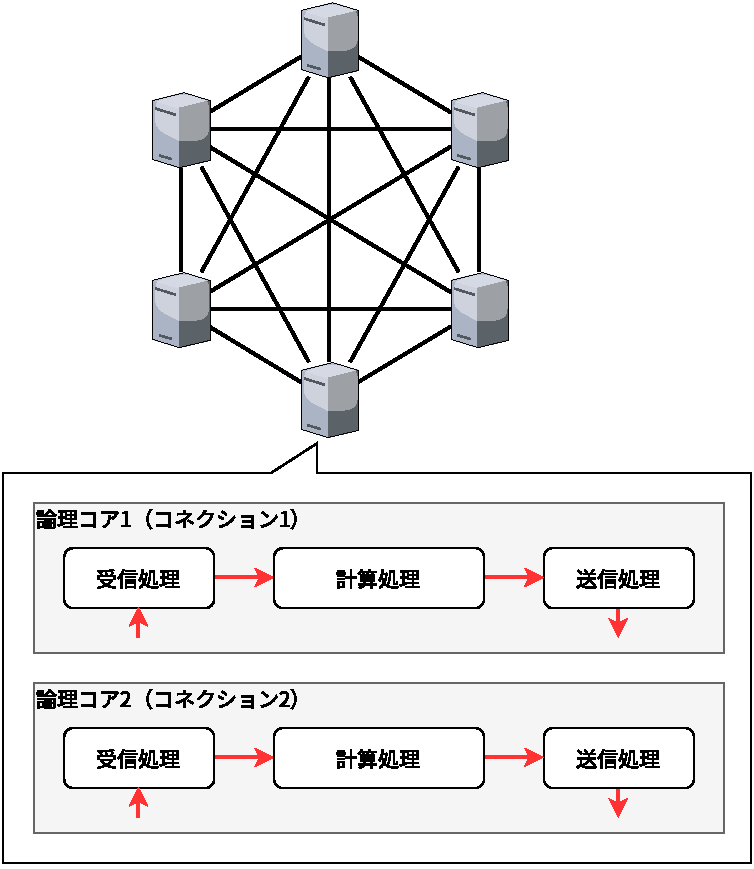
\includegraphics[width=\columnwidth]{pictures/Proposed.pdf}
  \caption{提案手法}
  \label{fig:Proposed}
\end{figure}

\section{事前実験1}
\label{sec:PreExperimentOne}
本章では,DPDKのRun-to-Completionモデルで実行する処理の負荷によって,スループットはどのように変化するかを調査するために行った事前実験1について述べる.

\subsection{事前実験1用のプログラム}
事前実験1用のプログラムとして,クライアントから送られてきたパケットを一定時間待機させてから送り返すプログラムを作成した(図\ref{fig:PreExperimentOne}).DPDKのRun-to-Completionモデルで実行する処理は,受信したパケットを待機させる処理である.パケットを待機させる時間を変更することにより,DPDKのRun-to-Completionモデルで実行する処理の負荷を仮想的に変更することができる.

\begin{figure}[htb]
  \centering
  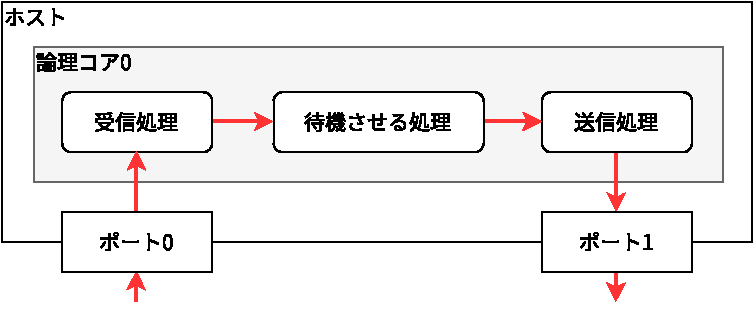
\includegraphics[width=\columnwidth]{pictures/PreExperimentOne.pdf}
  \caption{事前実験1用のプログラム}
  \label{fig:PreExperimentOne}
\end{figure}

\subsection{実験環境}
事前実験1で用いたネットワーク構成を図\ref{fig:PreExperimentNetwork}に示す.ホストAにおいてクライアントを動作させ,ホストBにおいて事前実験1用のプログラムを動作させた.クライアントには,DPDKベースのパケットジェネレータであるPktgen \cite{Pktgen} を用いた.事前実験1で用いた計算機の性能を表\ref{tab:MachineSpec},Pktgenの設定を表\ref{tab:PktgenSettings}に示す.

パケットはクライアントが動作するホストAのポート0から送信され,事前実験1用のプログラムが動作するホストBのポート0に到着する.到着したパケットは事前実験1用のプログラムによって待機させられてから,ホストBのポート1からホストAのポート1へと送り返される.

\begin{figure}[htb]
  \centering
  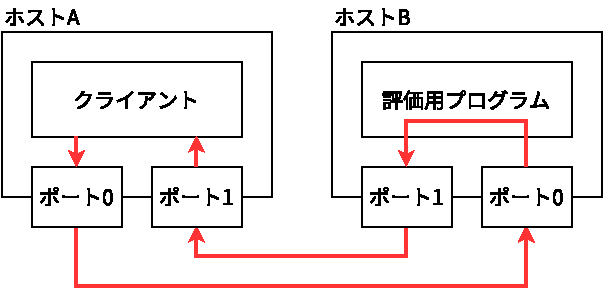
\includegraphics[width=\columnwidth]{pictures/PreExperimentNetwork.pdf}
  \caption{事前実験1で用いたネットワーク構成}
  \label{fig:PreExperimentNetwork}
\end{figure}

\begin{table}[htb]
  \centering
  \caption{事前実験1で用いた計算機の性能}
  \begin{tabular}{|c|c|} \hline
    OS     & Ubuntu 20.04                           \\ \hline
    CPU    & AMD Ryzen 5 3400G (4-cores, 8-threads) \\ \hline
    Memory & 16GB                                   \\ \hline
    NIC    & Intel X540-AT2 (10GbE, 2-ports)        \\ \hline
  \end{tabular}
  \label{tab:MachineSpec}
\end{table}

\begin{table}[htb]
  \centering
  \caption{Pktgenの設定}
  \begin{tabular}{|c|c|} \hline
    パケットのサイズ     & 64バイト, 128バイト \\ \hline
    送信するパケットの数 & 100,000,000パケット \\ \hline
    送信レート           & 100\%               \\ \hline
  \end{tabular}
  \label{tab:PktgenSettings}
\end{table}

\subsection{実験結果・考察}
事前実験1の結果を図\ref{fig:PreExperimentOneResult}に示す.このグラフの横軸はパケットの待機時間,縦軸は通信のスループットを表している.また,青はパケットサイズが64バイトのとき,赤はパケットサイズが128バイトのときの結果である.グラフより,パケットサイズが64バイトの場合,待機時間が1600ns以下のときスループットは一定であり,それを超えると単調減少することを確認した.また,パケットサイズが128バイトの場合,待機時間が3200ns以下のときスループットは一定であり,それを超えると単調減少することを確認した.よって,送信するパケットのサイズが小さく,送信レートが100\%という厳しい条件でも,処理時間が1600ns以下の計算処理であればスループットに影響を与えずにDPDKの送受信スレッドで実行できると考える.

\begin{figure}[htb]
  \centering
  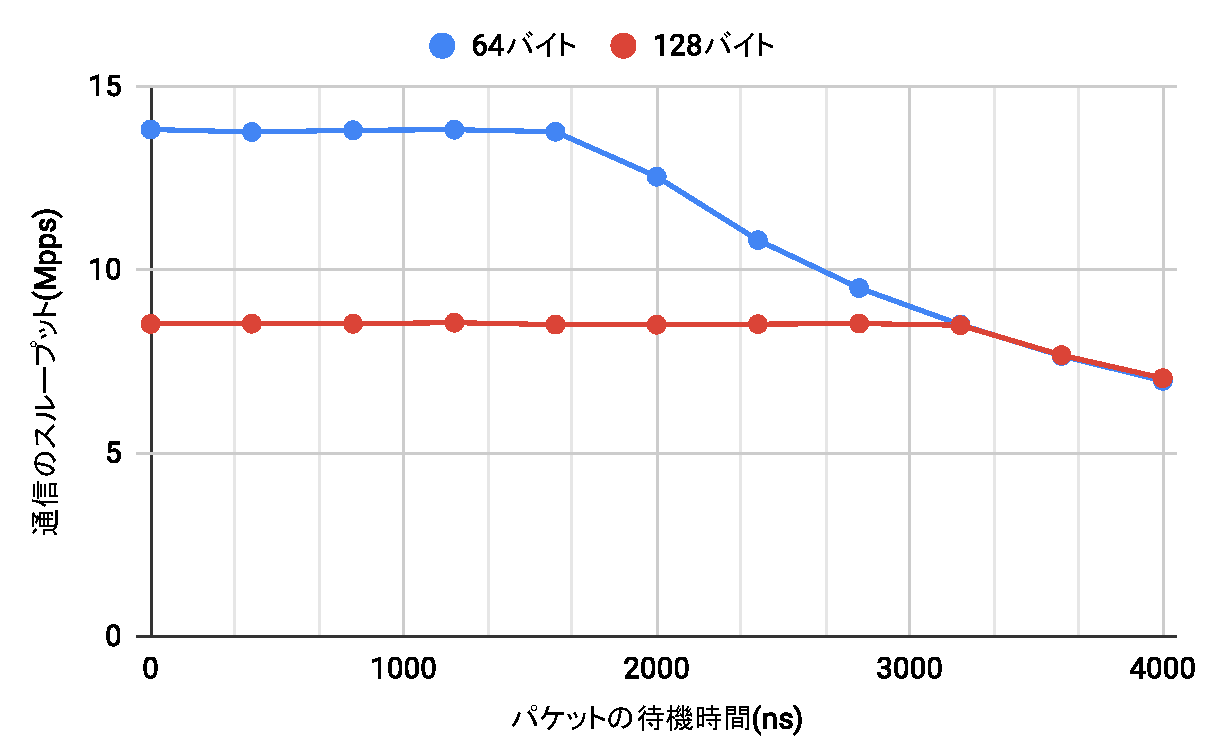
\includegraphics[width=\columnwidth]{pictures/PreExperimentOneResult.pdf}
  \caption{事前実験1の結果}
  \label{fig:PreExperimentOneResult}
\end{figure}

\section{事前実験2}
\label{sec:PreExperimentTwo}
事前実験2では,送られてきた32個の値を加算し送り返すプログラムにおいて,TCP/IPによる通信を用いる場合と提案手法を用いる場合の単位時間あたりの演算性能を比較した.

\subsection{事前実験2用のプログラム}
事前実験2用のプログラムとして,クライアントから送られてきた32個の値を加算し送り返すプログラムを作成した(図\ref{fig:PreExperimentTwo}).DPDKのRun-to-Completionモデルで実行する処理は受信したパケットに含まれる32個の値を加算する処理である.このプログラムはTCP/IPによる通信を用いる場合と提案手法を用いる場合の2種類を作成した.

\begin{figure}[htb]
  \centering
  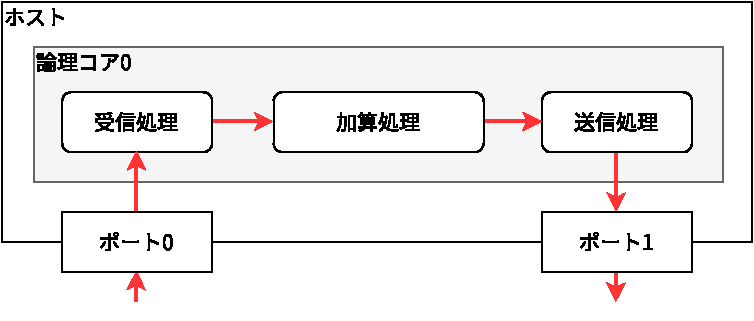
\includegraphics[width=\columnwidth]{pictures/PreExperimentTwo.pdf}
  \caption{事前実験2用のプログラム}
  \label{fig:PreExperimentTwo}
\end{figure}

\subsection{実験環境}
事前実験2で用いたネットワーク構成は事前実験1で用いたもの(図\ref{fig:PreExperimentNetwork})と同じである.ただし,クライアントにはパケットサイズが64バイトのパケットを送信レート100\%で送信し続ける自作プログラムを用いた.送信されるパケットのペイロードは要素数が32でデータ型がuint16\_tの配列である.なお,事前評価2で用いた計算機の性能は事前実験1で用いたもの(表\ref{tab:MachineSpec})と同じである.

\subsection{実験結果・考察}
事前実験2の結果を図\ref{fig:PreEvaluationTwoResult}に示す.このグラフの横軸は内部ループ回数,縦軸は単位時間あたりの演算性能を表している.また,青はTCP/IPによる通信を用いた場合,赤は提案手法を用いた場合の結果である.事前実験2用のプログラムでは,仮想的に内部演算量を増やすために,同一の加算処理を繰り返しており,その回数を内部ループ回数と定義する.グラフより,提案手法を用いた場合の演算性能はTCP/IPによる通信を用いた場合に比べて,内部ループ回数が1回の場合は30倍,10回の場合は4倍,100回の場合は0.4倍高いことを確認した.この結果より,分散計算環境において,DPDKによるL2通信を用いることとDPDKのRun-to-Completionモデルで処理を行うことは有効であると考える.なお,提案手法を用いた場合の演算性能が内部ループ回数が多くなるにつれて低下する理由は,計算処理量の増加により受信処理に割り当てられるCPUリソースが相対的に減少したためであると考える.

\begin{figure}[htb]
  \centering
  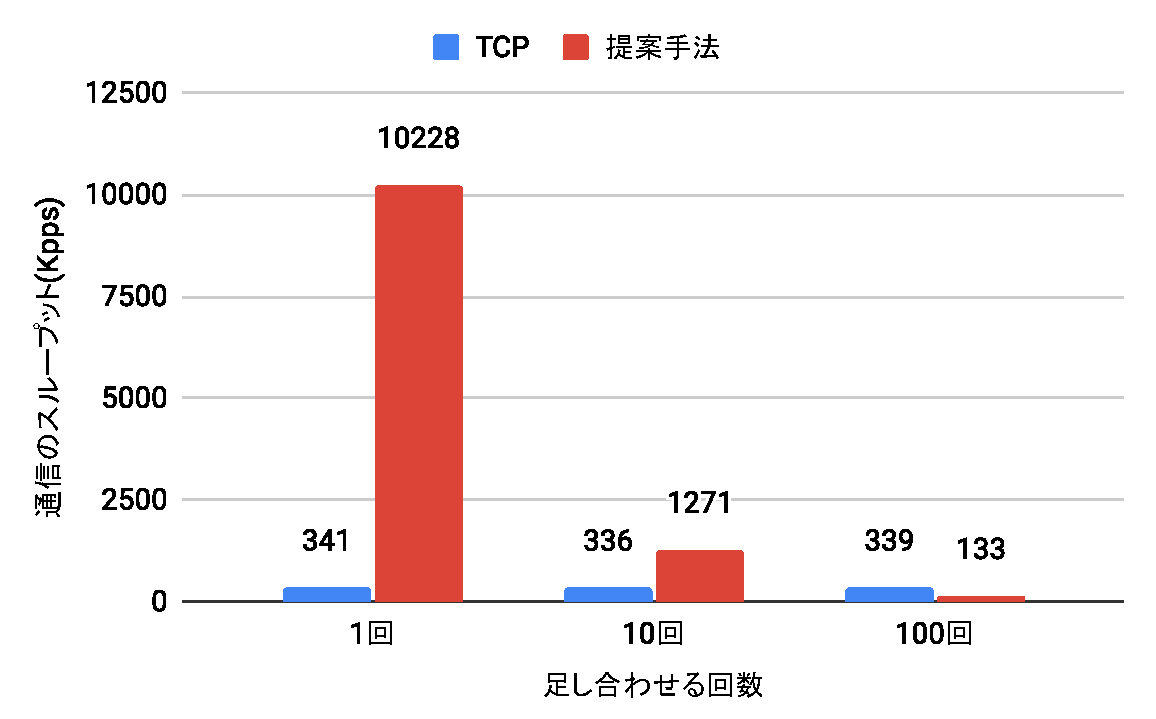
\includegraphics[width=\columnwidth]{pictures/PreExperimentTwoResult.pdf}
  \caption{加算処理の結果}
  \label{fig:PreEvaluationTwoResult}
\end{figure}

\section{評価}
\label{sec:Evaluation}
本章では,提案手法の有効性を確認するために行った評価について述べる.評価では,単回帰分析において,1台での集中学習を行う場合,TCP/IPによる通信を用いた分散学習を行う場合,提案手法を用いた分散学習を行う場合の実行時間を比較した.

\subsection{評価用プログラム}
評価用プログラムとして単回帰分析を行うプログラムを作成した.単回帰分析とは,与えられたデータを用いて$y = ax + b$の傾き$a$と切片$b$を求める問題である.パラメータの最適化には確率的勾配降下法(Stochastic Gradient Descent, SGD)を用いた.確率的勾配降下法とは,データをランダムに選んで以下の更新を繰り返し,$f$を最小化するアルゴリズムである.なお,パラメータを$w$,学習率を$\alpha$,目的関数を$f$とする.

\begin{equation}
  w \leftarrow w - \alpha \nabla f(w)
\end{equation}

複数台の計算機で分散して学習を行う場合はパラメータの集約が必要となる.パラメータの集約にはGossip Learning \cite{Gossip1}, \cite{Gossip2} を用いた.Gossip Learningにおいて,各計算機は確率的勾配降下法によってパラメータを更新する.そして,定期的にランダムに選んだ他の計算機と通信し,パラメータの平均を計算する.このようなパラメータの更新を繰り返していくことによって学習が進む.

このプログラムは1台での集中学習を行うもの,TCP/IPによる通信を用いた分散学習を行うもの,提案手法を用いた分散学習を行うものの3種類を作成した.

\subsection{評価環境}
評価で用いたネットワーク構成を図\ref{fig:Evaluation}に示す.計算機を接続し,それぞれの計算機で評価用プログラムを動作させた.なお,評価で用いた計算機の性能は事前実験1で用いたもの(表\ref{tab:MachineSpec})と同じである.

\begin{figure}[htb]
  \centering
  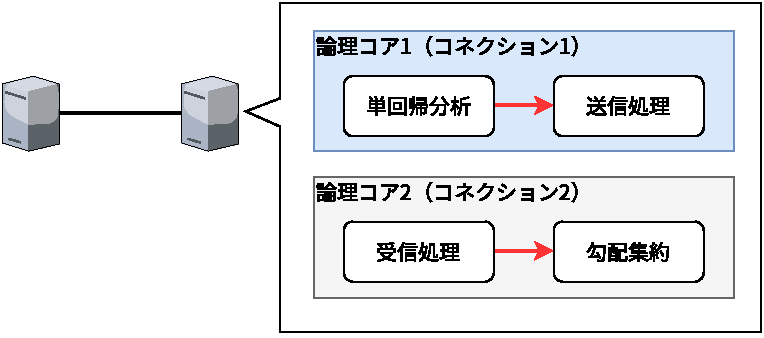
\includegraphics[width=\columnwidth]{pictures/EvaluationNetwork.pdf}
  \caption{評価で用いたネットワーク構成}
  \label{fig:Evaluation}
\end{figure}

\subsection{評価結果・考察}
評価結果を図\ref{fig:EvaluationResult}に示す.このグラフの横軸は左から1台での集中学習の場合,TCP/IPによる通信を用いた2台での分散学習の場合,提案手法を用いた2台での分散学習の場合を表しており,縦軸は実行時間を表している.グラフより,提案手法を用いた2台での分散学習の実行時間は,1台での集中学習の場合に比べて2倍,TCP/IPによる通信を用いた2台での分散学習の場合に比べて1.2倍高速であることを確認した.よって,分散計算環境において,DPDKによるL2通信を用いることとDPDKのRun-to-Completionモデルで処理を行うことは有効であると考える.

\begin{figure}[htb]
  \centering
  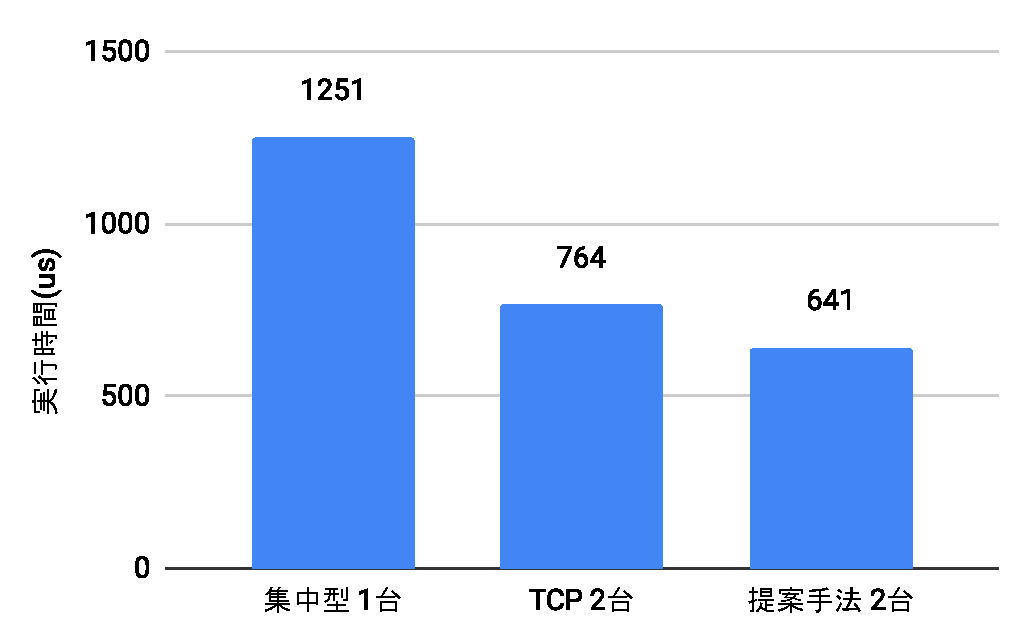
\includegraphics[width=\columnwidth]{pictures/EvaluationResult.pdf}
  \caption{評価結果}
  \label{fig:EvaluationResult}
\end{figure}

\section{関連研究}
\label{sec:RelatedWorks}
多元連立一次方程式の緩和法解析の分散処理にDPDKによる通信を用いる研究 \cite{RelaxationMethodDPDK} がある.1992年に小石らによって行われた多元連立一次方程式の緩和法解析の分散処理に関する研究 \cite{RelaxationMethodUDP} では,UDPによるブロードキャストが行われていた.そこで,文献 \cite{RelaxationMethodDPDK} では多元連立一次方程式の緩和法解析の分散処理にDPDKを用いることで,通信オーバーヘッドの削減による計算の高速化を行った.その結果,DPDKを用いた緩和法解析の分散処理アプリケーションは,UDPを用いた分散処理よりも最大40.1\%高速化された.しかし,文献 \cite{RelaxationMethodDPDK} では受信スレッド,収束判定または計算のスレッド,送信スレッドのそれぞれが論理コアを使用するPipelineモデルを用いているため,CPUリソースやL1キャッシュを有効活用できない.

MPI通信のデータ転送にDPDKを用いる研究 \cite{MPIDPDK} がある.多くのMPIライブラリはデータ転送を行うレイヤが独立しており,ユーザの環境に合わせてデータ転送方式やデバイスをMPIプログラムの実行に柔軟に切り替えることができる.そこで,文献 \cite{MPIDPDK} はMPIライブラリの新たなデータ転送モジュールとしてDPDKによるデータ転送モジュールを提案した.通信のスループットが低いときはRun-to-Completionモデル,高いときはPipelineモデルを使用するようになっている.その結果,TCP/IPソケットによるデータ転送を用いた場合と比べ,通信遅延を最大77\%改善することができた.しかし,この研究ではACKパケットの授受を実装することによって,パケットロスに対する制御を行っているため,通信のオーバーヘッドがある.

\section{まとめと今後の課題}
\label{sec:Conclusion}
本稿では,DPDKのRun-to-Completionモデルを用いたL2分散計算環境を提案した.計算機間の通信にDPDKによるL2通信を用いることによって,TCP/IPによる通信のオーバーヘッドを低減するとともに,カーネルによるパケットI/O処理に比べて高速なパケットI/O処理を用いることができる.また,Run-to-Completionモデルを採用することによって,Pipelineモデルを用いる場合に比べてCPUリソースやL1キャッシュを有効活用できる.送られてきた32個の値を加算し送り返すプログラムを用いた事前実験2では,提案手法を用いた場合の処理性能はTCP/IPによる通信を用いた場合に比べて,内部ループ回数が1回の場合は30倍,10回の場合は4倍,100回の場合は0.4倍高いことを確認した.また,単回帰分析を行うプログラムを用いた評価では,提案手法を用いた2台での分散学習の実行時間は,1台での集中学習の場合に比べて2倍,TCP/IPによる通信を用いた2台での分散学習の場合に比べて1.2倍高速であることを確認した.

今後の課題としては,使用する計算機の台数を増やして評価を取ること,提案手法のどの部分が性能向上に寄与しているのかを調べるためにRaw Socketを用いてカーネルによるL2通信を実装して評価を取ること,ロジスティック回帰やサポートベクターマシン(Support Vector Machine, SVM)といった複雑な機械学習を実行することなどがある.


\begin{acknowledgment}
  本研究の一部は,科研費基盤研究(C)22K12048による.
\end{acknowledgment}

\bibliographystyle{ipsjunsrt}
\bibliography{Thesis}

\end{document}
